\documentclass[]{article}
\usepackage[margin=2cm]{geometry}

%opening
\title{Exercises Set: Differential Equations\\ \large Solutions}
\author{DSBA Mathematics Refresher 2026}
\date{}

\usepackage{amsmath}
\usepackage{amsfonts}
\usepackage{amsthm}
\usepackage{amssymb}
\usepackage{mathrsfs}
\usepackage{stmaryrd}
\usepackage{tikz}

\newcommand{\Q}{\mathbb{Q}}
\newcommand{\N}{\mathbb{N}}
\newcommand{\Z}{\mathbb{Z}}
\newcommand{\R}{\mathbb{R}}
\newcommand{\Primes}{\mathbb{P}}
\newcommand{\st}{\text{ s.t. }}
\newcommand{\txtand}{\text{ and }}
\newcommand{\txtor}{\text{ or }}
\newcommand{\lxor}{\veebar}


\begin{document}

	\maketitle

	\section{First Order Differential Equations}
	\paragraph{Basics}\mbox{}

	\textbf{Exercise 0:} $\dfrac{dy}{dx} = 3x^2 - 2x + 1$.

	Integrating both sides with respect to $x$:
	$$y = x^3 - x^2 + x + C, \qquad C \in \R$$

	\textbf{Exercise 1:} $\dfrac{dy}{dx} = 5y$.

	Try $y = \alpha e^{\beta x}$; then $y' = \alpha\beta e^{\beta x} = \beta y$, so we need $\beta = 5$:
	$$y = \alpha e^{5x}, \qquad \alpha \in \R$$
	With the condition $y(0) = 2$: $\alpha e^{0} = \alpha = 2$, hence
	$$y = 2 e^{5x}$$

	\begin{center}
		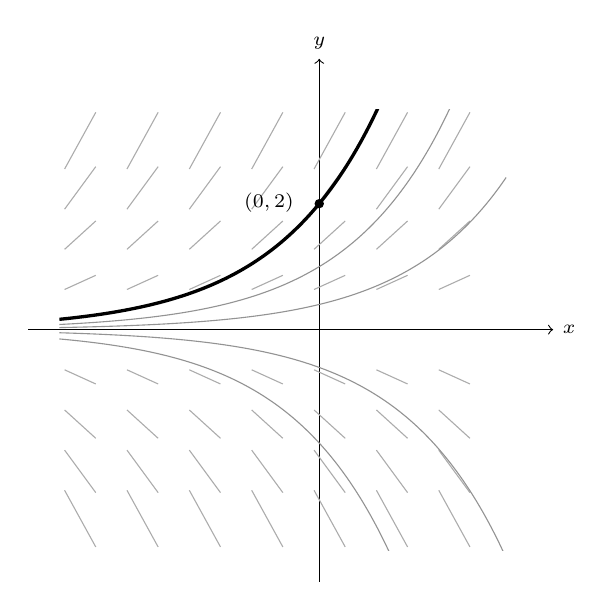
\begin{tikzpicture}[xscale=6.6,yscale=0.8]
			\draw[->] (-0.56,0) -- (0.45,0) node[right] {\scriptsize $x$};
			\draw[->] (0,-4.0) -- (0,4.3) node[above] {\scriptsize $y$};
			\begin{scope}
				\clip (-0.5,-3.5) rectangle (0.36,3.5);
				\foreach \a in {-0.46,-0.34,-0.22,-0.10,0.02,0.14,0.26}{
					\foreach \b in {-3,-2.25,-1.5,-0.75,0.75,1.5,2.25,3}{
						\draw[gray!65] ({\a-0.030},{\b-0.15*\b}) -- ({\a+0.030},{\b+0.15*\b});
					}
				}
				\draw[gray!85,domain=-0.5:0.36,samples=60,smooth] plot ({\x},{0.4*exp(5*\x)});
				\draw[gray!85,domain=-0.5:0.36,samples=60,smooth] plot ({\x},{1*exp(5*\x)});
				\draw[gray!85,domain=-0.5:0.36,samples=60,smooth] plot ({\x},{-0.6*exp(5*\x)});
				\draw[gray!85,domain=-0.5:0.36,samples=60,smooth] plot ({\x},{-1.8*exp(5*\x)});
				\draw[very thick,domain=-0.5:0.36,samples=60,smooth] plot ({\x},{2*exp(5*\x)});
			\end{scope}
			\node[circle,fill,minimum size=3.4pt,inner sep=0] at (0,2) {};
			\node[left] at (-0.03,2.02) {\scriptsize $(0,2)$};
		\end{tikzpicture}
	\end{center}
	The short grey segments show the slope $5y$ imposed by the equation at each point --- the \textbf{direction field}.
	Every solution must follow it, and the grey curves are four members of the family $y = \alpha e^{5x}$.
	They never cross: through each point of the plane passes exactly one of them.
	The initial condition $y(0) = 2$ simply picks out the one through the marked point (in black).

	\paragraph{Separable}\mbox{}

	\textbf{Exercise 2:} $\dfrac{dy}{dx} = \dfrac{x}{y}$.

	Separating the variables and integrating:
	\begin{align*}
		y \, dy &= x \, dx \\
		\int y \, dy &= \int x \, dx \\
		\tfrac{1}{2} y^2 &= \tfrac{1}{2} x^2 + \tfrac{C}{2}, \qquad C \in \R \\
		y^2 &= x^2 + C
	\end{align*}
	so $y = \pm\sqrt{x^2 + C}$ (on any interval where $x^2 + C > 0$).

	\textit{Check:} $y' = \pm\dfrac{2x}{2\sqrt{x^2+C}} = \pm\dfrac{x}{\sqrt{x^2+C}} = \dfrac{x}{y}$. \checkmark

	\textbf{Exercise 3:} $\dfrac{dy}{dx} = 2x^2 e^y$.

	Separating the variables and integrating:
	\begin{align*}
		e^{-y} \, dy &= 2x^2 \, dx \\
		\int e^{-y} \, dy &= \int 2x^2 \, dx \\
		-e^{-y} &= \tfrac{2}{3} x^3 - C, \qquad C \in \R \\
		e^{-y} &= C - \tfrac{2}{3} x^3
	\end{align*}
	so, taking logarithms,
	$$y = -\ln\!\left(C - \tfrac{2}{3}x^3\right)$$
	valid on any interval where $C - \tfrac{2}{3}x^3 > 0$.

	\paragraph{Integrating Factor}\mbox{}

	\textbf{Exercise 4:} $y' + 2y = 4x$.

	The integrating factor is $\mathrm{IF} = e^{\int 2 \, dx} = e^{2x}$. Multiplying the equation by it:
	\begin{align*}
		y' e^{2x} + 2y e^{2x} &= 4x e^{2x} \\
		\left(y e^{2x}\right)' &= 4x e^{2x} \\
		y e^{2x} &= \int 4x e^{2x} \, dx = 2x e^{2x} - e^{2x} + C, \qquad C \in \R
	\end{align*}
	(the integral is done by parts), so
	$$y = 2x - 1 + C e^{-2x}$$

	\textit{Check:} $y' = 2 - 2Ce^{-2x}$, hence $y' + 2y = 2 - 2Ce^{-2x} + 4x - 2 + 2Ce^{-2x} = 4x$. \checkmark

	\textbf{Exercise 5: (*)} $y' - \dfrac{1}{x} y = x^3$.

	Working on $x > 0$, the integrating factor is $\mathrm{IF} = e^{\int -\frac{1}{x} dx} = e^{-\ln(x)} = \dfrac{1}{x}$. Multiplying by it:
	\begin{align*}
		\frac{1}{x} y' - \frac{1}{x^2} y &= x^3 \cdot \frac{1}{x} = x^2 \\
		\left(\frac{y}{x}\right)' &= x^2 \\
		\frac{y}{x} &= \frac{1}{3} x^3 + C, \qquad C \in \R
	\end{align*}
	so
	$$y = \frac{1}{3} x^4 + C x$$

	\textit{Check:} $y' = \dfrac{4}{3}x^3 + C$, hence $y' - \dfrac{1}{x} y = \dfrac{4}{3}x^3 + C - \dfrac{1}{3}x^3 - C = x^3$. \checkmark



	\section{Second Order Differential Equations}
	\paragraph{Basics}\mbox{}

	\textbf{Exercise 0:} $y'' = e^x + 4\sin(2x) - 5x$.

	Integrating once:
	$$y' = e^x - 2\cos(2x) - \tfrac{5}{2} x^2 + C, \qquad C \in \R$$
	Integrating a second time:
	$$y = e^x - \sin(2x) - \tfrac{5}{6} x^3 + Cx + D, \qquad C, D \in \R$$

	\textbf{Exercise 1:} $y'' + 2y' + y = 0$.

	Assume $y = e^{rx}$; then $r^2 e^{rx} + 2r e^{rx} + e^{rx} = 0$, i.e.
	$$r^2 + 2r + 1 = 0 \quad \Longleftrightarrow \quad (r+1)^2 = 0 \quad \Longleftrightarrow \quad r = -1 \ \text{(double root)}$$
	So $y = A e^{-x}$ is a solution. Since the root is double, we also try $y = x e^{rx}$:
	$$y' = r x e^{rx} + e^{rx}, \qquad y'' = r^2 x e^{rx} + 2r e^{rx}$$
	$$y'' + 2y' + y = x e^{rx}\left(r^2 + 2r + 1\right) + e^{rx}\left(2r + 2\right) = 0$$
	which again holds for $r = -1$. Hence $y = B x e^{-x}$ is a solution too, and in general
	$$y = A e^{-x} + B x e^{-x} = (A + Bx) e^{-x}, \qquad A, B \in \R$$

	\textbf{Exercise 2:} $y'' + 4y = 0$.

	With $y = e^{rx}$ we get $r^2 + 4 = 0$, so $r = \pm 2i$ and
	\begin{align*}
		y &= A e^{2ix} + B e^{-2ix} \\
		  &= A\left(\cos(2x) + i\sin(2x)\right) + B\left(\cos(2x) - i\sin(2x)\right)
	\end{align*}
	Letting $C = A + B$ and $D = (A - B) i$, the real solutions are
	$$y = C \cos(2x) + D \sin(2x), \qquad C, D \in \R$$

	\begin{center}
		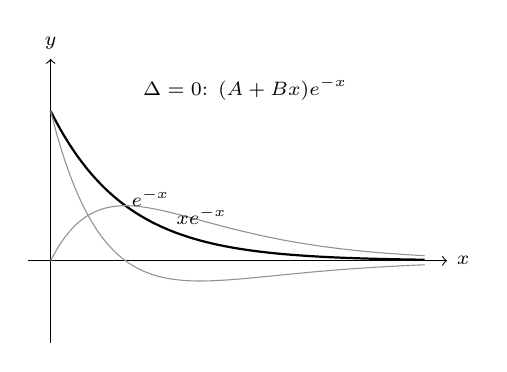
\begin{tikzpicture}[xscale=0.95,yscale=1.9]
			\draw[->] (-0.3,0) -- (5.3,0) node[right] {\scriptsize $x$};
			\draw[->] (0,-0.55) -- (0,1.35) node[above] {\scriptsize $y$};
			\draw[thick,domain=0:5,samples=60,smooth] plot ({\x},{exp(-\x)});
			\draw[gray!85,domain=0:5,samples=60,smooth] plot ({\x},{\x*exp(-\x)});
			\draw[gray!85,domain=0:5,samples=60,smooth] plot ({\x},{(1-\x)*exp(-\x)});
			\node at (2.6,1.15) {\scriptsize $\Delta = 0$: $(A+Bx)e^{-x}$};
			\node[right] at (0.95,0.42) {\scriptsize $e^{-x}$};
			\node[right] at (1.55,0.30) {\scriptsize $xe^{-x}$};
		\end{tikzpicture}
		\hspace{4mm}
		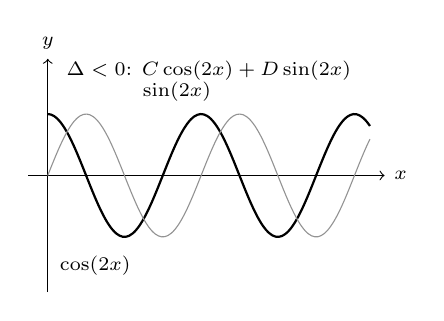
\begin{tikzpicture}[xscale=0.62,yscale=0.78]
			\draw[->] (-0.4,0) -- (6.9,0) node[right] {\scriptsize $x$};
			\draw[->] (0,-1.9) -- (0,1.9) node[above] {\scriptsize $y$};
			\draw[thick,domain=0:6.6,samples=100,smooth] plot ({\x},{cos(2*\x r)});
			\draw[gray!85,domain=0:6.6,samples=100,smooth] plot ({\x},{sin(2*\x r)});
			\node at (3.3,1.7) {\scriptsize $\Delta < 0$: $C\cos(2x)+D\sin(2x)$};
			\node[below right] at (0.05,-1.15) {\scriptsize $\cos(2x)$};
			\node[above right] at (1.75,1.05) {\scriptsize $\sin(2x)$};
		\end{tikzpicture}
	\end{center}
	The sign of the discriminant is visible in the shape of the solutions: a real root gives pure
	\textit{decay} (left, with the extra factor $x$ allowing one bump before it dies out), while a pair of
	complex roots gives \textit{oscillation} (right).
	Here $\alpha = 0$, so the oscillation neither grows nor decays; a non-zero real part would multiply
	these curves by $e^{\alpha x}$ and make them spiral out or die away.

	\paragraph{Separable}\mbox{}

	\textbf{Exercise 3:} $y'' = (y')^2$.

	Let $z = y' = \dfrac{dy}{dx}$. The equation becomes $z' = z^2$, which is separable:
	\begin{align*}
		\frac{dz}{z^2} &= dx \\
		\int \frac{dz}{z^2} &= \int dx \\
		-\frac{1}{z} &= x + C, \qquad C \in \R \\
		z &= -\frac{1}{x + C}
	\end{align*}
	Then $\dfrac{dy}{dx} = -\dfrac{1}{x+C}$, so integrating once more:
	$$y = -\ln|x + C| + D, \qquad C, D \in \R$$

	\textit{Check:} $y' = -\dfrac{1}{x+C}$ and $y'' = \dfrac{1}{(x+C)^2} = (y')^2$. \checkmark

	(Note that the constant functions $y = D$ are solutions as well.)

	\paragraph{Non-homogeneous}\mbox{}

	\textbf{Exercise 4:} $y'' + 4y' + 4y = 6x^2 + 10x + 2$.

	\textit{Homogeneous equation:} $r^2 + 4r + 4 = 0$, i.e. $(r+2)^2 = 0$, so $r = -2$ is a double root and
	$$y_{\text{hom}} = A e^{-2x} + B x e^{-2x}, \qquad A, B \in \R$$

	\textit{Particular solution:} the right-hand side is a degree-2 polynomial, so we look for $y = a x^2 + b x + c$. Then $y' = 2ax + b$ and $y'' = 2a$, so
	$$y'' + 4y' + 4y = 4a x^2 + (8a + 4b) x + (2a + 4b + 4c)$$
	Identifying coefficients with $6x^2 + 10x + 2$:
	$$\begin{cases}
		4a = 6 \\
		8a + 4b = 10 \\
		2a + 4b + 4c = 2
	\end{cases}
	\quad \Longrightarrow \quad
	a = \frac{3}{2}, \quad b = -\frac{1}{2}, \quad c = \frac{1}{4}$$
	so $y_{\text{part}} = \dfrac{3}{2} x^2 - \dfrac{1}{2} x + \dfrac{1}{4}$.

	\textit{General solution:}
	$$y = y_{\text{hom}} + y_{\text{part}} = A e^{-2x} + B x e^{-2x} + \frac{3}{2} x^2 - \frac{1}{2} x + \frac{1}{4}$$

	\textbf{Exercise 5:} $y'' - 2y' + 5y = 3 e^{2t}$.

	\textit{Homogeneous equation:} $r^2 - 2r + 5 = 0$, with $\Delta = 4 - 20 = -16$, so $r = 1 \pm 2i$ and
	$$y_{\text{hom}} = A e^{(1+2i)t} + B e^{(1-2i)t} = e^{t}\left(C \cos(2t) + D \sin(2t)\right), \qquad C, D \in \R$$

	\textit{Particular solution:} try $y = a e^{2t}$; then
	$$y'' - 2y' + 5y = e^{2t}\left(4a - 4a + 5a\right) = 5a\, e^{2t}$$
	so $5a = 3$, i.e. $a = \dfrac{3}{5}$ and $y_{\text{part}} = \dfrac{3}{5} e^{2t}$.

	\textit{General solution:}
	$$y = e^{t}\left(C \cos(2t) + D \sin(2t)\right) + \frac{3}{5} e^{2t}$$

	\paragraph{Boundary Conditions}\mbox{}

	\textbf{Exercise 6:} $y'' + 2y' - 3y = 0$, with $y(0) = 0$ and $y(2) = 5$.

	\textit{Homogeneous equation:} $r^2 + 2r - 3 = 0$, with $\Delta = 4 + 12 = 16$, so $r = \dfrac{-2 \pm 4}{2}$, i.e. $r = 1$ or $r = -3$:
	$$y = A e^{x} + B e^{-3x}, \qquad A, B \in \R$$

	\textit{Boundary conditions:}
	$$y(0) = 0 \quad \Longrightarrow \quad A + B = 0 \quad \Longrightarrow \quad B = -A$$
	$$y(2) = 5 \quad \Longrightarrow \quad A e^{2} + B e^{-6} = A\left(e^{2} - e^{-6}\right) = 5 \quad \Longrightarrow \quad A = \frac{5}{e^{2} - e^{-6}}$$
	Finally,
	$$y = \frac{5}{e^{2} - e^{-6}} \, e^{x} - \frac{5}{e^{2} - e^{-6}} \, e^{-3x} = \frac{5\left(e^{x} - e^{-3x}\right)}{e^{2} - e^{-6}}$$

	\textit{Check:} $y(0) = 0$ \checkmark \ and $y(2) = \dfrac{5(e^2 - e^{-6})}{e^2 - e^{-6}} = 5$. \checkmark

	\textbf{Exercise 7: (*)} $y'' + 4y = 12x$, with $y(0) = 0$ and $y'(0) = 2$.

	\textit{Homogeneous equation:} as in Exercise 2 above,
	$$y_{\text{hom}} = C \cos(2x) + D \sin(2x), \qquad C, D \in \R$$

	\textit{Particular solution:} try $y = ax + b$; then $y'' = 0$ and $y'' + 4y = 4ax + 4b$, so $4a = 12$ and $4b = 0$, giving $y_{\text{part}} = 3x$.

	\textit{General solution:}
	$$y = C \cos(2x) + D \sin(2x) + 3x$$

	\textit{Boundary conditions:}
	$$y(0) = 0 \quad \Longrightarrow \quad C = 0$$
	$$y'(x) = -2C \sin(2x) + 2D \cos(2x) + 3, \quad \text{so} \quad y'(0) = 2D + 3 = 2 \quad \Longrightarrow \quad D = -\frac{1}{2}$$
	Finally,
	$$y = -\frac{1}{2} \sin(2x) + 3x$$

	\textit{Check:} $y' = -\cos(2x) + 3$ and $y'' = 2\sin(2x)$, so $y'' + 4y = 2\sin(2x) - 2\sin(2x) + 12x = 12x$ \checkmark, \ $y(0) = 0$ \checkmark, \ $y'(0) = -1 + 3 = 2$. \checkmark

\end{document}
